\chapter{Resultados obtenidos y análisis}
\label{cap:rt_resultados_y_analisis}

En el presente capítulo se exponen y analizan los datos recolectados del experimento en tiempo real (véase el Capítulo \ref{cap:experimentoTiempoReal}), con el objetivo de evaluar el funcionamiento de la arquitectura y sacar conclusiones en base a ello.

Debido a que el experimento se ha realizado con una muestra reducida de tres
participantes, el enfoque de este análisis prioriza la observación detallada e
individualizada de cada caso. A continuación, se exponen los resultados
objetivos extraídos de las grabaciones y los datos subjetivos de los
formularios.

\section{Perfilado de los participantes}
\label{sec:rt_perfiles}

A continuación se presenta una breve descripción de los participantes en forma
de tabla (ver la Tabla \ref{tab:sujetos}).

Cabe destacar, a modo de aclaración, que el sujeto 3 tenía el pelo más corto de
longitud a la hora del experimento que el resto. Asimismo, la densidad capilar
del sujeto 3 también es menor que las del sujeto 1 y 2 (a pesar de que el
sujeto 1 también la tenga baja).

Como notas adicionales, todos los participantes optaron por utilizar el
dispositivo de ejercitación ofrecido (como se menciona en las
\hyperref[subsec:rt_instrucciones]{instrucciones al participante}). El
participante que más aprovechó este recurso fue el sujeto 3, mientras que el 1
y el 2 lo usaron menos.

\begin{table}[h]
      \centering
      \begin{tabular}{|c|c|c|c|}
            \hline
            \textbf{Característica}   & \textbf{Sujeto 1} & \textbf{Sujeto 2} & \textbf{Sujeto 3} \\
            \hline

            Edad                      & 21                & 21                & 22                \\ \hline Sexo & H & H & H \\ \hline Dominancia manual &
            Diestro                   & Diestro           & Diestro                               \\ \hline Densidad capilar & Baja & Media & Baja \\
            \hline Experiencia con MI & Poca              & Ninguna           & Ninguna           \\ \hline Problemas
            neurológicos              & No                & Migrañas con aura & No                \\ \hline

      \end{tabular}
      \caption{Características de los sujetos}
      \label{tab:sujetos}
\end{table}

\section{Evaluación del sistema base (\textit{benchmark} visual)}
\label{sec:rt_res_benchmark}
En la Tabla \ref{tab:resultados_benchmark} se exponen los tiempos medios de reacción de cada usuario durante la fase de \textit{benchmark}, midiendo la consistencia en el flujo de predicciones puras antes de entrar a los entornos dinámicos de los videojuegos.

\begin{table}[h!]
      \centering
      \resizebox{\textwidth}{!}{
            \begin{tabular}{|l|c|c|c|}
                  \hline
                  \textbf{Participante} & \textbf{Tiempo medio iteración (s)} & \textbf{Experiencia previa} \\ \hline
                  Sujeto 1              & 11,65                               & Sí                          \\ \hline
                  Sujeto 2              & 12,05                               & No                          \\ \hline
                  Sujeto 3              & 7,16                                & No                          \\ \hline
            \end{tabular}
      }
      \caption{Tiempos de reacción en el \textit{benchmark} visual (\textit{dualArrowComponent}).}
      \label{tab:resultados_benchmark}
\end{table}

\section{Rendimiento en videojuegos}
\label{sec:rt_res_videojuegos}

En esta sección se agrupan las métricas numéricas explicadas anteriormente,
todas se han obtenido de los vídeos.

\subsection{Tiempos máximos de supervivencia}

En la Tabla \ref{tab:tiempos_supervivencia} se exponen la mejor racha de cada
jugador para los distintos escenarios. Destaca por encima de todos el sujeto 3
en el juego \textit{wave runner} con 1 minuto y 10 segundos.

\begin{table}[h!]
      \centering
      \begin{tabular}{|l|c|c|c|c|c|c|}
            \hline
            \multirow{2}{*}{\textbf{Participante}} & \multicolumn{2}{c|}{\textbf{Wave Runner (s)}} & \multicolumn{2}{c|}{\textbf{Project Arrows (s)}}                                         \\ \cline{2-5}
                                                   & \textbf{Ayuda 0}                              & \textbf{Ayuda 0,7}                               & \textbf{Ayuda 0} & \textbf{Ayuda 0,7} \\ \hline
            Sujeto 1                               & 8,47                                          & \textbf{63,10}                                   & 19,60            & \textbf{27,58}     \\ \hline
            Sujeto 2                               & 23,42                                         & \textbf{51,45}                                   & 30,00            & \textbf{35,90}     \\ \hline
            Sujeto 3                               & 30,14                                         & \textbf{70,00}                                   & 41,6             & \textbf{57,13}     \\ \hline
      \end{tabular}
      \caption{Tiempo máximo sobrevivido por usuario, videojuego y nivel de asistencia. No se incluyen los tiempos para el nivel de asistencia 1. Se resalta con negrita el valor máximo por cada juego y participante.}
      \label{tab:tiempos_supervivencia}
\end{table}

\subsection{Tiempo medio de reacción ante obstáculos}

A continuación se muestran las medias calculadas con los tiempos de reacción de
cada sujeto, por juego y nivel de ayuda (ver Tabla
\ref{tab:tiempos_supervivencia}).

\begin{table}[h!]
      \centering
      \begin{tabular}{|l|c|c|c|c|c|c|}
            \hline
            \multirow{2}{*}{\textbf{Participante}} & \multicolumn{2}{c|}{\textbf{Wave Runner (s)}} & \multicolumn{2}{c|}{\textbf{Project Arrows (s)}}                                       \\ \cline{2-5}
                                                   & \textbf{Ayuda 0}                              & \textbf{Ayuda 0,7}                               & \textbf{Ayuda} & \textbf{Ayuda 0,7} \\ \hline
            Sujeto 1                               & 1,82                                          & 4,17                                             & 3,19           & 2,63               \\ \hline
            Sujeto 2                               & 4,53                                          & 4,94                                             & 2,29           & 2,42               \\ \hline
            Sujeto 3                               & 3,39                                          & 4,74                                             & 2,09           & 2,52               \\ \hline
      \end{tabular}
      \caption{Tiempo medio de reacción ante obstáculos por usuario, videojuego y nivel de asistencia.}
      \label{tab:tiempos_medios}
\end{table}

\subsection{Tasas de aciertos}

Por último, en la Tabla \ref{tab:tasas_aciertos} se pueden ver los porcentajes
de acierto que han tenido los usuarios por juego y ayuda.

\begin{table}[h!]
      \centering
      \begin{tabular}{|l|c|c|c|c|c|c|}
            \hline
            \multirow{2}{*}{\textbf{Participante}} & \multicolumn{2}{c|}{\textbf{Wave Runner (\%)}} & \multicolumn{2}{c|}{\textbf{Project Arrows (\%)}}                                         \\ \cline{2-5}
                                                   & \textbf{Ayuda 0}                               & \textbf{Ayuda 0,7}                                & \textbf{Ayuda 0} & \textbf{Ayuda 0,7} \\ \hline
            Sujeto 1                               & 36,80                                          & 74,44                                             & 50,00            & 77,78              \\ \hline
            Sujeto 2                               & 47,72                                          & 77,19                                             & 75,00            & 83,34              \\ \hline
            Sujeto 3                               & 51,56                                          & 79,17                                             & 72,5             & 86,27              \\ \hline
      \end{tabular}
      \caption{Tasa de obstáculos superados frente al número de obstáculos afrontados por usuario, videojuego y nivel de asistencia.}
      \label{tab:tasas_aciertos}
\end{table}

\section{Experiencia de usuario}
\label{sec:rt_res_formulario}
% Aquí analizas las respuestas del formulario. Al ser 3 personas, puedes decir cosas como: "La totalidad de los sujetos reportó diversión..." o "Dos de los tres participantes sintieron frustración con la latencia...". 
% Se recomienda hacer un gráfico de barras apiladas o radar con las respuestas de la escala Likert.
Se han recolectado los datos del formulario de todos los participantes para cada sesión de juego y se han obtenido los resultados que se muestran en las
Figuras \ref{fig:Preguntas_formulario_1} a \ref{fig:Preguntas_formulario_10}.
En cada una de estas figuras se muestra la distribución de respuestas elegidas
por nivel de ayuda para cada pregunta, viéndose representadas en los mismos
colores que se muestran en la leyenda.

\begin{figure}[h]
      \centering
      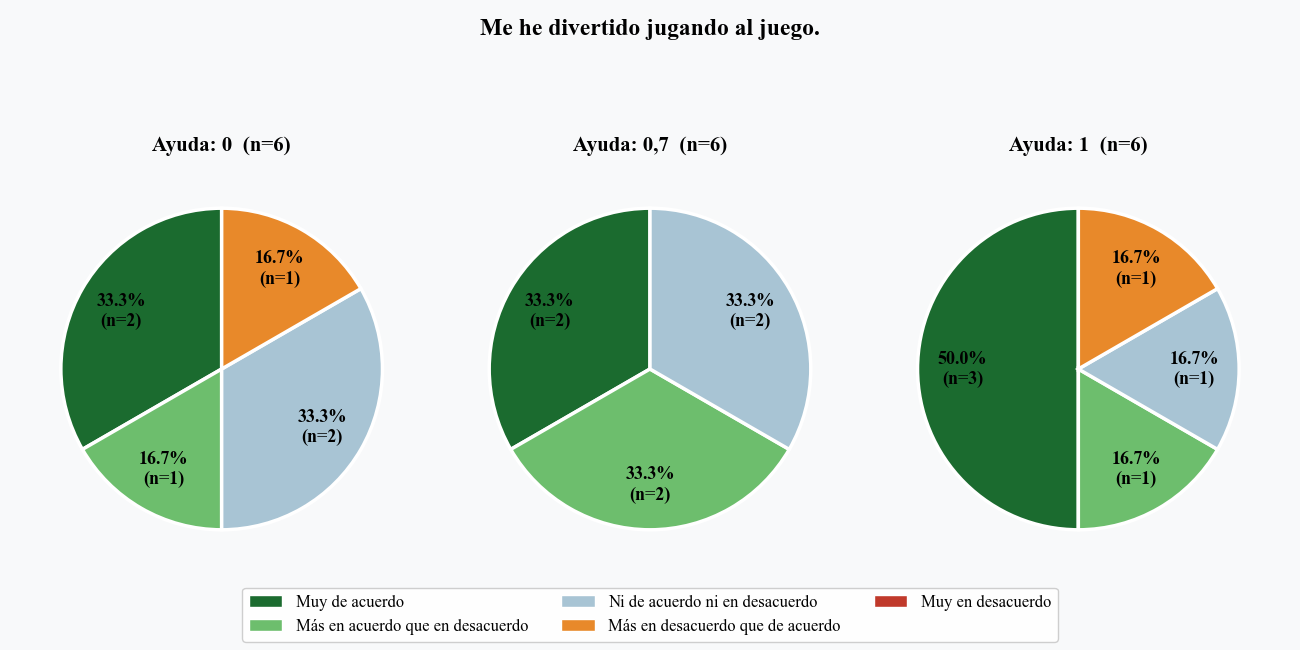
\includegraphics[width=1\textwidth]{Imagenes/Bitmap/Formulario_Pregunta_1.png}
      \caption{Distribución de respuestas por nivel de ayuda de la pregunta 1: ``Me he divertido jugando al juego''.}
      \label{fig:Preguntas_formulario_1}
\end{figure}

\begin{figure}[h]
      \centering
      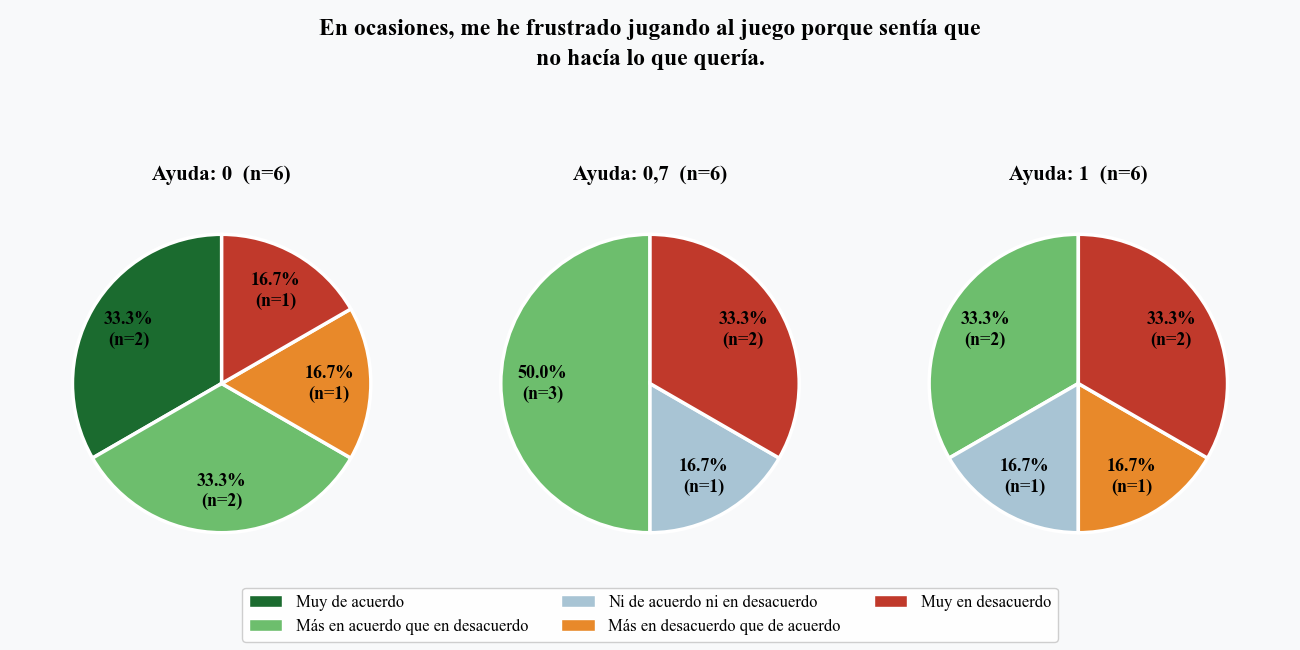
\includegraphics[width=1\textwidth]{Imagenes/Bitmap/Formulario_Pregunta_2.png}
      \caption{Distribución de respuestas por nivel de ayuda de la pregunta 2: ``En ocasiones, me he frustrado jugando al juego porque sentía que no hacía lo que quería''.}
      \label{fig:Preguntas_formulario_2}
\end{figure}

\begin{figure}[h]
      \centering
      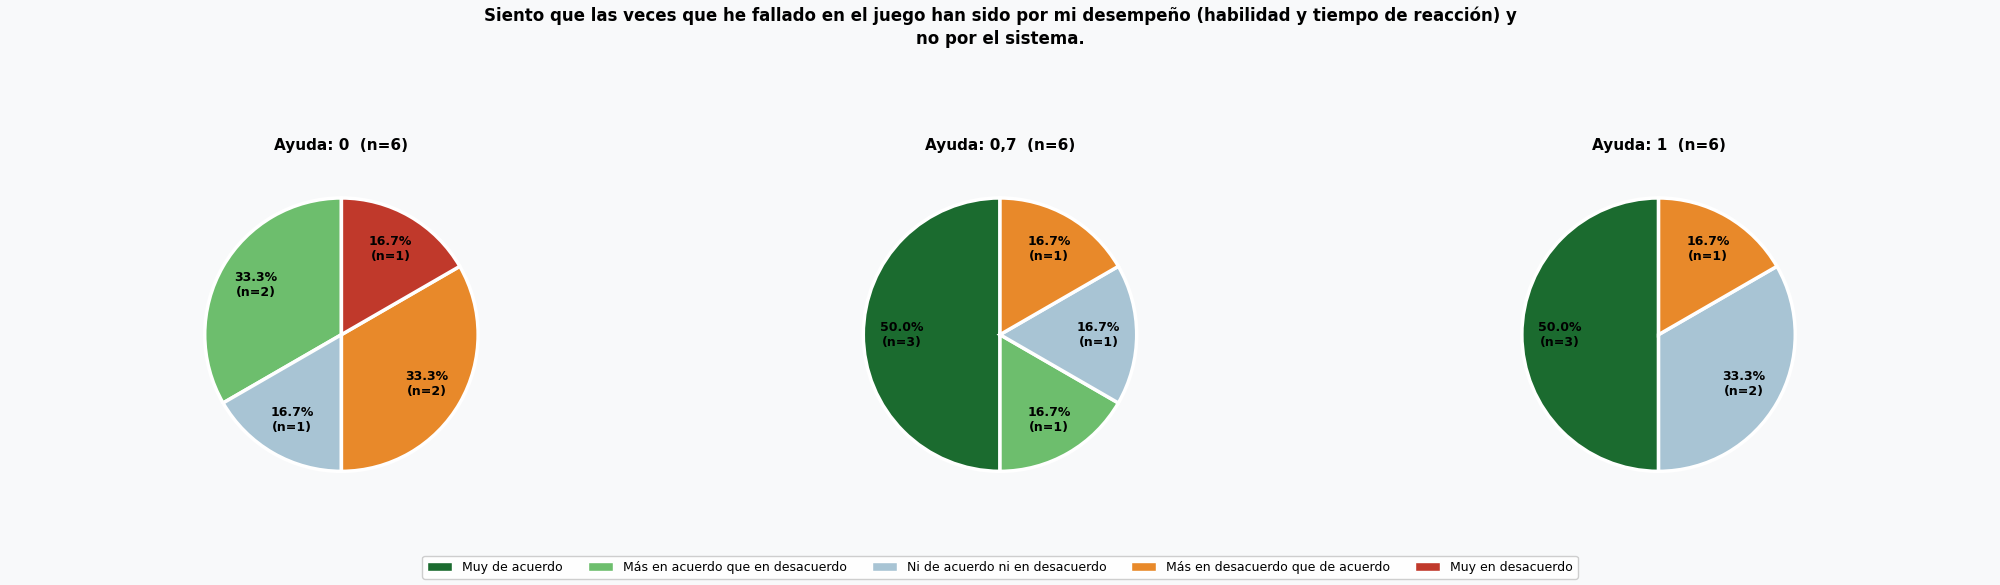
\includegraphics[width=1\textwidth]{Imagenes/Bitmap/Formulario_Pregunta_3.png}
      \caption{Distribución de respuestas por nivel de ayuda de la pregunta 3: ``Siento que las veces que he fallado en el juego han sido por mi desempeño (habilidad y tiempo de reacción) y no por el sistema''.}
      \label{fig:Preguntas_formulario_3}
\end{figure}

\begin{figure}[h]
      \centering
      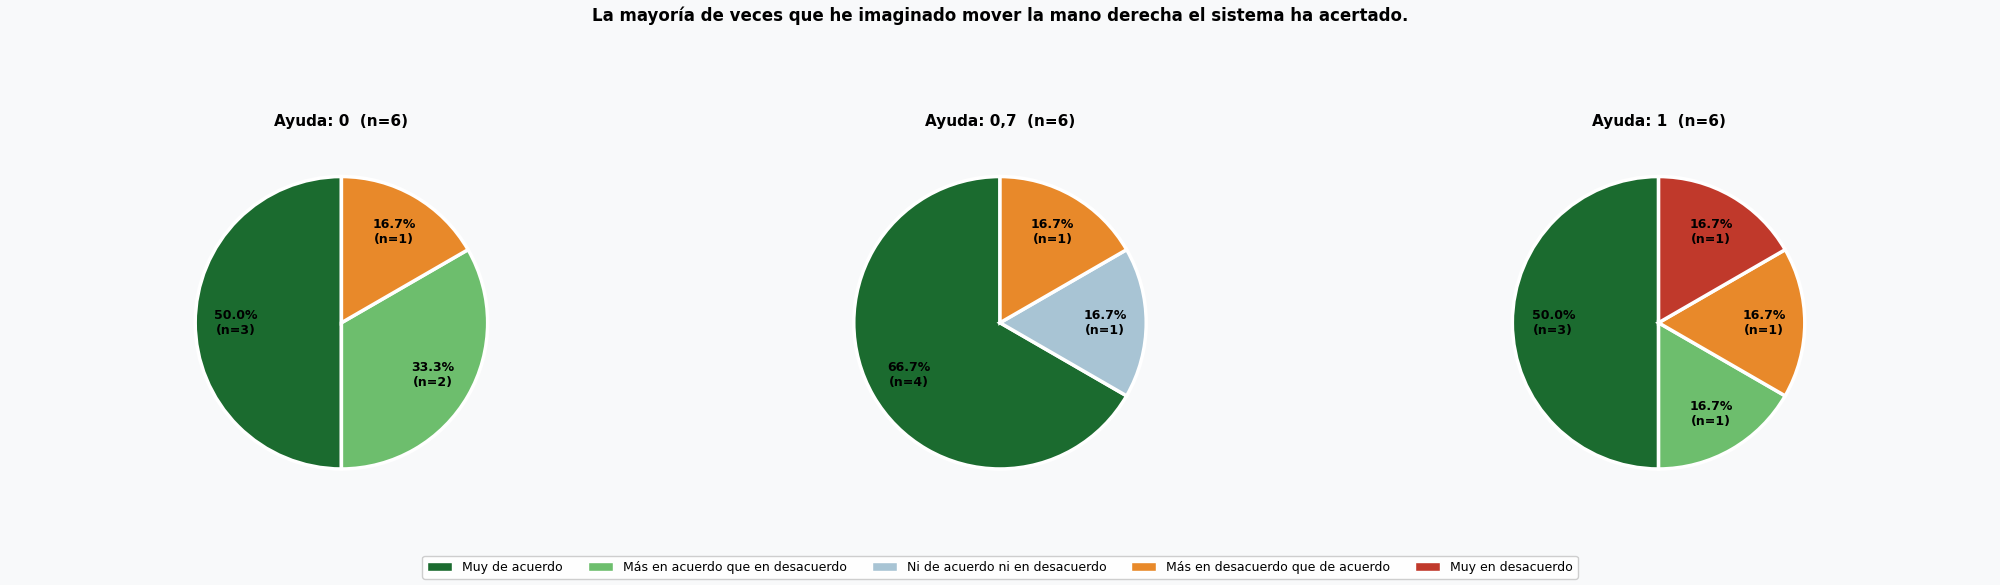
\includegraphics[width=1\textwidth]{Imagenes/Bitmap/Formulario_Pregunta_4.png}
      \caption{Distribución de respuestas por nivel de ayuda de la pregunta 4: ``La mayoría de veces que he imaginado mover la mano derecha el sistema ha acertado''.}
      \label{fig:Preguntas_formulario_4}
\end{figure}

\begin{figure}[h]
      \centering
      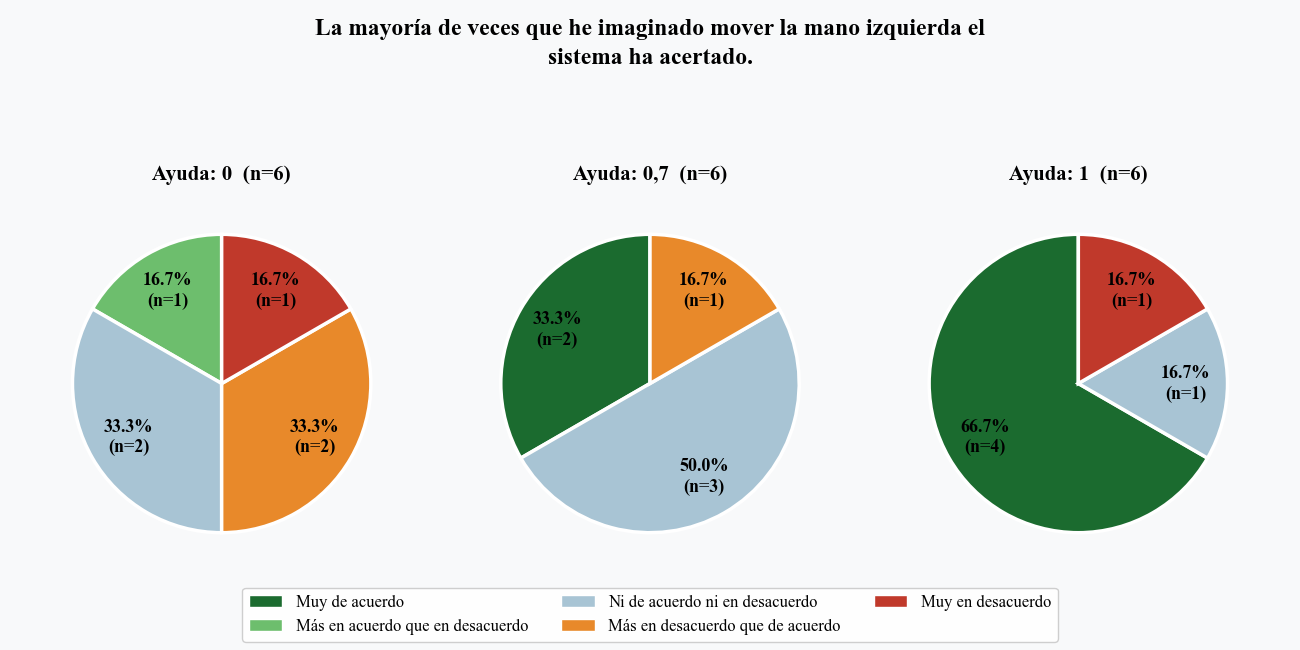
\includegraphics[width=1\textwidth]{Imagenes/Bitmap/Formulario_Pregunta_5.png}
      \caption{Distribución de respuestas por nivel de ayuda de la pregunta 5: ``La mayoría de veces que he imaginado mover la mano izquierda el sistema ha acertado''.}
      \label{fig:Preguntas_formulario_5}
\end{figure}

\begin{figure}[h]
      \centering
      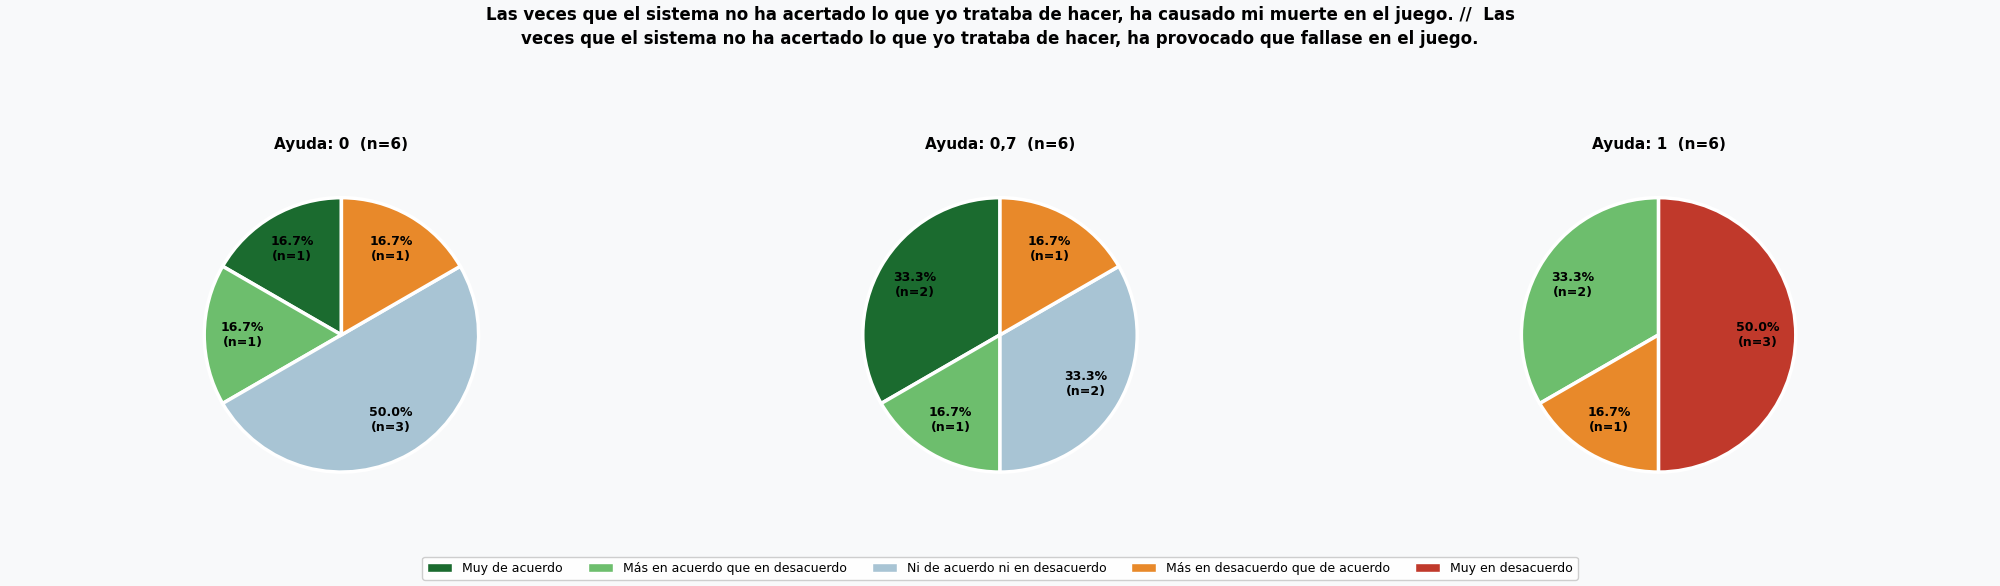
\includegraphics[width=1\textwidth]{Imagenes/Bitmap/Formulario_Pregunta_6.png}
      \caption{Distribución de respuestas por nivel de ayuda de la pregunta 6: ``He notado latencia (retardo) desde que trataba de hacer una acción hasta que se tomaba realmente''.}
      \label{fig:Preguntas_formulario_6}
\end{figure}

\begin{figure}[h]
      \centering
      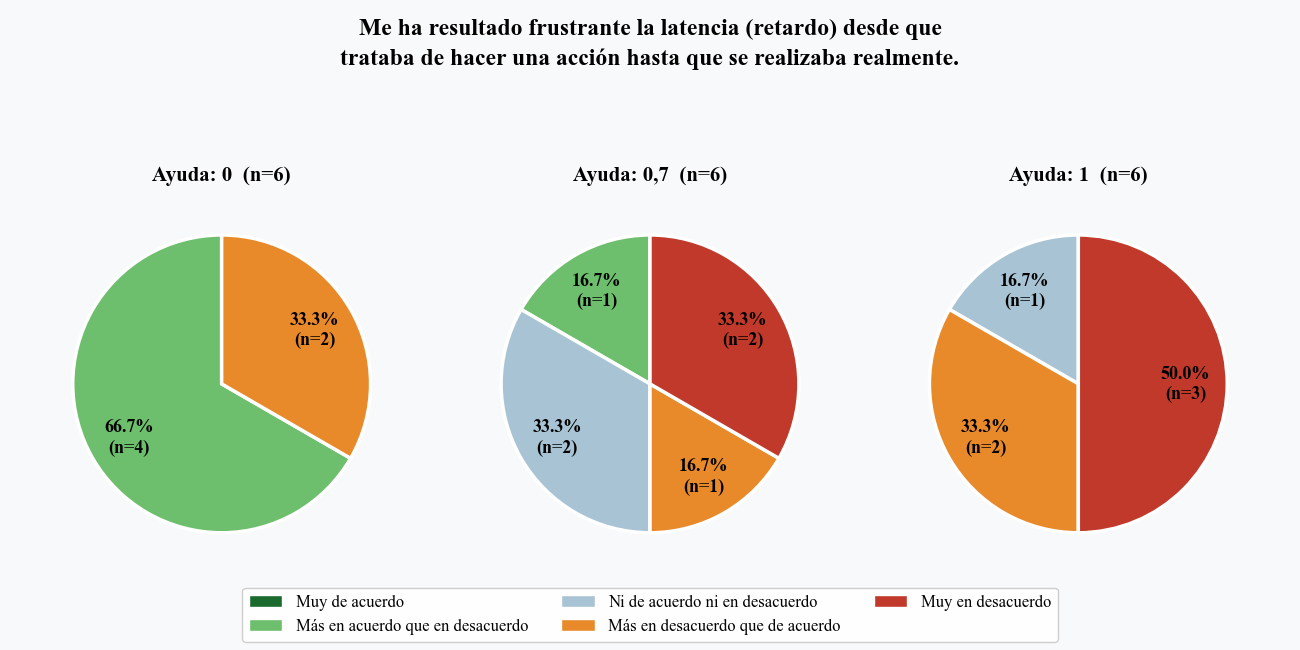
\includegraphics[width=1\textwidth]{Imagenes/Bitmap/Formulario_Pregunta_7.png}
      \caption{Distribución de respuestas por nivel de ayuda de la pregunta 7: ``Me ha resultado frustrante la latencia (retardo) desde que trataba de hacer una acción hasta que se realizaba realmente''.}
      \label{fig:Preguntas_formulario_7}
\end{figure}

\begin{figure}[h]
      \centering
      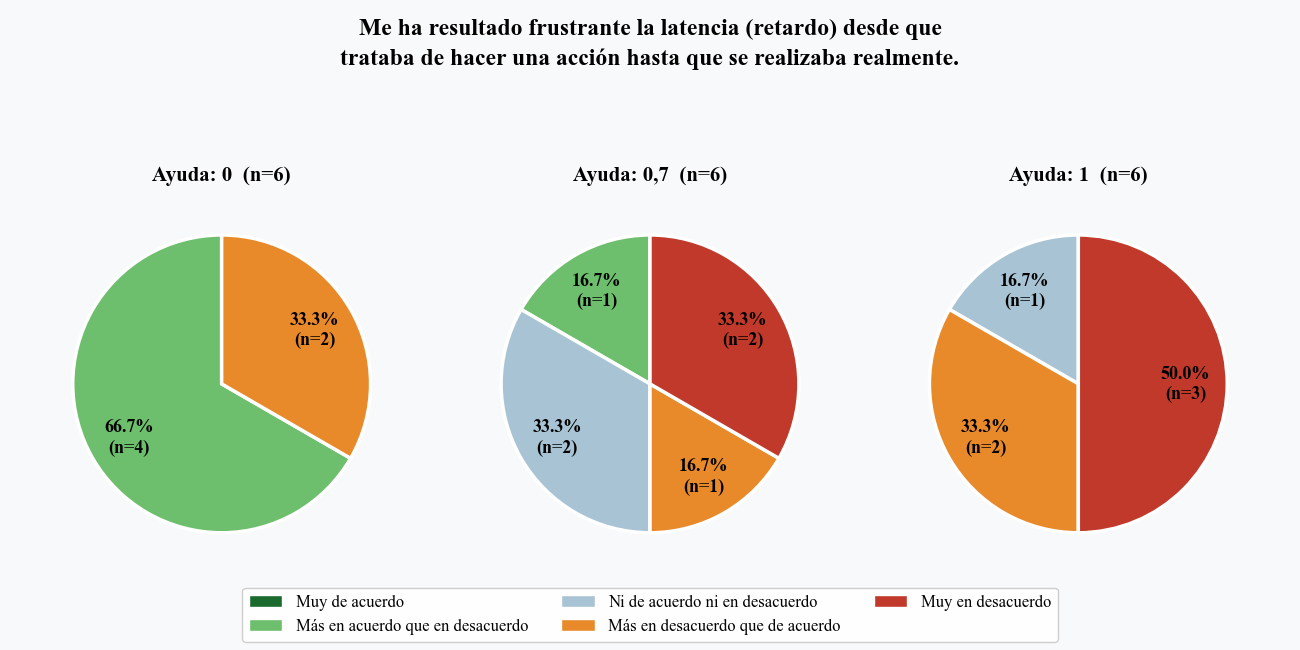
\includegraphics[width=1\textwidth]{Imagenes/Bitmap/Formulario_Pregunta_8.png}
      \caption{Distribución de respuestas por nivel de ayuda de la pregunta 8: ``Me ha parecido que la velocidad del juego era acorde a la velocidad de las acciones que podía tomar''.}
      \label{fig:Preguntas_formulario_8}
\end{figure}

\begin{figure}[h]
      \centering
      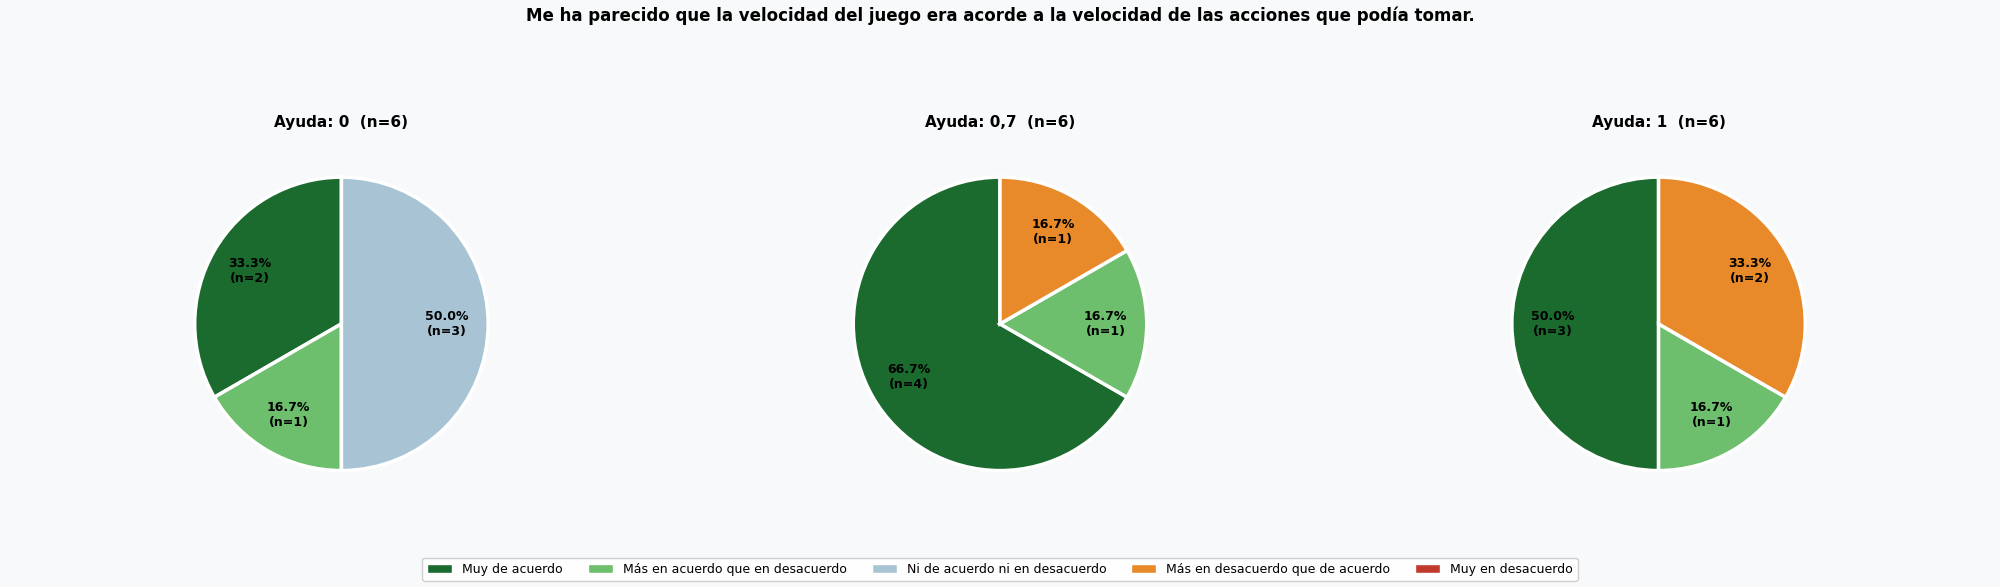
\includegraphics[width=1\textwidth]{Imagenes/Bitmap/Formulario_Pregunta_9.png}
      \caption{Distribución de respuestas por nivel de ayuda de la pregunta 9: ``Me ha resultado demasiado lenta la velocidad del juego, hasta el punto de frustrarme''.}
      \label{fig:Preguntas_formulario_9}
\end{figure}

\begin{figure}[h]
      \centering
      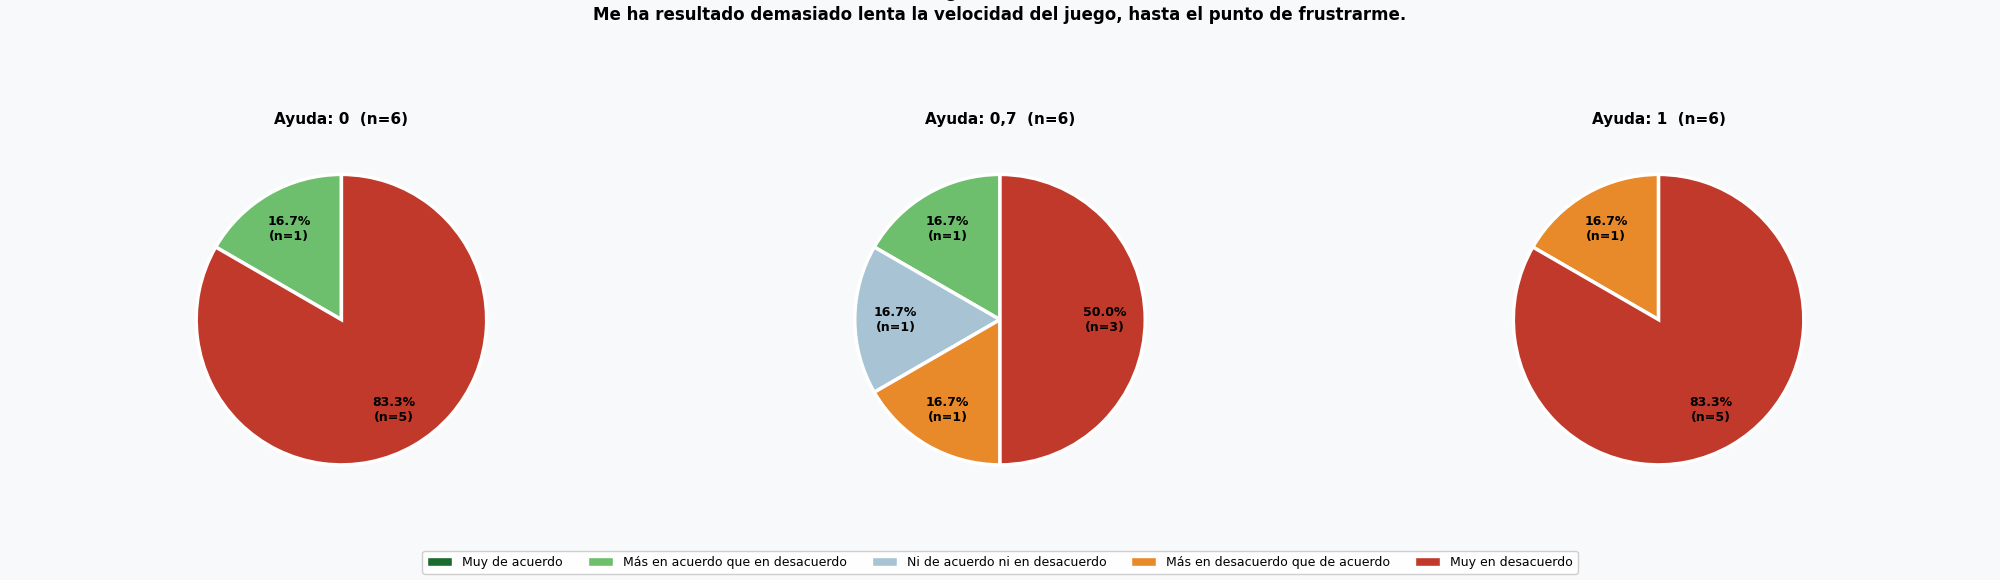
\includegraphics[width=1\textwidth]{Imagenes/Bitmap/Formulario_Pregunta_10.png}
      \caption{Distribución de respuestas por nivel de ayuda de la pregunta 10: ``En general, estoy satisfecho con el desempeño del sistema y la experiencia de juego''.}
      \label{fig:Preguntas_formulario_10}
\end{figure}

\section{Análisis de los resultados obtenidos}
\label{sec:rt_analisis_aislado}
A partir de los datos obtenidos para las métricas de rendimiento y las respuestas al formulario, se procede a realizar una análisis claro que permita comprender el desempeño del sistema y de los participantes.

\subsection{Evaluación del sistema base (\textit{benchmark} visual)}
\label{subsec:rt_analisis_benchmark}

Tomando como referencia la Tabla \ref{tab:resultados_benchmark} se puede
observar que el sujeto 3 parte de una mejor base a la hora de controlar el
sistema, con una diferencia de entre 4 y 5 segundos frente al resto de
participantes.

Esta diferencia resulta impactante teniendo en cuenta que el sujeto 1 dispone
de experiencia previa con MI. Sin embargo, es importante recordar que el sujeto
3 tenía una menor densidad y longitud capilar que el resto. Como observación
adicional, este sujeto fue el que más utilizó el mecanismo de entrenamiento de
mano y antebrazo.

Es posible que el rendimiento del sujeto 3 esté justificado por estos dos
factores.

\subsection{Tiempos máximos de supervivencia}
\label{subsec:rt_analisis_tiempos_maximos}

Analizando la Tabla \ref{tab:tiempos_supervivencia}, se puede observar una
clara mejora de los tiempos cuando se activa la ayuda al nivel 0,7 frente a
deshabilitarla. Este es un resultado esperado, los filtros de ayuda (véase la
Subsección \ref{subsec:filtros_ayuda}) están ideados y diseñados con el
objetivo de mejorar el desempeño de los sujetos en los videojuegos.

El sujeto que más se ha beneficiado de esta ayuda según la tabla ha sido el 1,
con una mejoría de 55 segundos aproximadamente en el juego \textit{wave
      runner}.

Al igual que anteriormente, el sujeto 3 presenta los mejores resultados.
Teniendo mejores tiempos que los demás participantes para ambos juegos, con y
sin filtro de ayuda.

Como observación adicional, los tiempos máximos para el juego \textit{wave
      runner} son, por lo general, mayores que para el juego \textit{project arrows}.
Esto se debe a la naturaleza de los juegos, más que al funcionamiento del
sistema o al rendimiento de los usuarios: el \textit{project arrows} resulta un
videojuego más rápido, obligando a tomar decisiones en menor tiempo; mientras
que el \textit{wave runner} deja algo más de margen normalmente.

\subsection{Tiempo medio de reacción ante obstáculos}
\label{subsec:rt_analisis_tiempos_maximos}

Contemplando la Tabla \ref{tab:tiempos_medios}, se observa un incremento del
tiempo de reacción tras aplicar la ayuda en el videojuego \textit{wave runner}.
Para entender esto, se debe tener en cuenta que los tiempos de reacción no
dejan de ser una estimación: no se puede saber con exactitud cuándo ha pensado
el usuario en realizar la acción realmente, así que se toma como referencia el
momento en el que el peligro se hace claro (véase el
\hyperref[subsec:protocoloObtencionMetricas]{protocolo de obtención de
      métricas}). Además, por la naturaleza del juego resulta beneficioso una
reacción más retardada, siempre y cuando el jugador no se choque (en el
\textit{wave runner} si cambias de lado instantes antes de chocarte, tienes
mayor margen para reaccionar antes de chocarte con la otra pared).

Es por esto mismo que, en el \textit{wave runner} se relacionan tiempos altos
de supervivencia (véase la Tabla \ref{tab:tiempos_supervivencia}) con tiempos
medios de reacción elevados.

Un factor a tener en cuenta para el \textit{wave runner} es que, en ocasiones
el usuario muere tratando de reaccionar a un peligro y al reaparecer continua
ese peligro activo. Por tanto, se pueden presentar tiempos más bajos de lo
normal. Es por esto que el sujeto 1 tiene el menor tiempo de reacción de media
en este juego y sin ayuda (1,82) a pesar de tener el peor rendimiento (véanse
las tablas \ref{tab:tiempos_supervivencia} y \ref{tab:tasas_aciertos})

Por otro lado, los los tiempos para \textit{project arrows} resultan muy
similares con y sin ayuda. Esto también se puede relacionar a la naturaleza del
propio juego, ya que en cuanto el jugador supera un obstáculo, se le aproxima
otro en un corto periodo de tiempo.

Por último, es importante destacar que las mediciones de esta métrica se han
tomado en base a los tiempos de los obstáculos superados, sin añadir ninguna
penalización al valor medio para los casos en el que el obstáculo no ha sido
superado.

\subsection{Tasas de aciertos}
\label{subsec:rt_analisis_tasas_aciertos}

La Tabla \ref{tab:tasas_aciertos} nos muestra claramente que el filtro de ayuda
aplicado mejora considerablemente el porcentaje de aciertos, independientemente
del usuario y del juego, consiguiendo hasta mejoras de entre 30 y 40 porciento
en algunos casos.

Se puede observar también que los participantes 2 y 3 han obtenido tasas
similares en los distintos escenarios. Mientras que el sujeto 1 presenta un
peor desempeño sin ayuda, pero se asemeja a los otros dos una vez aplicado el
filtro de asistencia.

\subsection{Experiencia de usuario}
\label{subsec:rt_analisis_experiencia_usuario}

\begin{enumerate}
      \item \textbf{Diversión del participante al utilizar el sistema.} Para esta categoría de preguntas se han tomado las preguntas y sus respectivas gráficas en las figuras: \ref{fig:Preguntas_formulario_1} y \ref{fig:Preguntas_formulario_2}.

            \begin{itemize}
                  \item \textbf{Sin ayuda:} En las sesiones sin asistencia, los
                        participantes reportan una experiencia de juego menos satisfactoria,
                        atribuible a la frustración generada por el retardo en la respuesta y la
                        acumulación de fallos. Si bien una parte de los participantes afirma haber
                        disfrutado de la experiencia, las respuestas relativas a la frustración
                        revelan una tendencia clara hacia la percepción de falta de control sobre
                        el juego.
                  \item \textbf{Ayuda de 0,7:} Este nivel de asistencia refleja una
                        mejora notable en la experiencia de usuario. Las respuestas se desplazan
                        hacia valoraciones más positivas en cuanto a disfrute, sin que ningún
                        participante haya manifestado no haberse divertido. No obstante, en lo
                        relativo a la frustración, las opiniones se mantienen divididas, con una
                        parte considerable de los participantes que aún percibe cierta falta de
                        control sobre el juego, lo que sugiere que este nivel de ayuda, aunque
                        óptimo en términos de disfrute, no elimina completamente la sensación de
                        frustración.
                  \item \textbf{Ayuda de 1:} Con el máximo nivel de asistencia, los
                        resultados son en general similares a los del nivel 0.7, aunque se aprecia
                        alguna respuesta discordante en cuanto al disfrute de la partida. En
                        contrapartida, las valoraciones sobre la frustración por falta de control
                        se desplazan mayoritariamente hacia el desacuerdo o la neutralidad, lo que
                        indica que, pese a que el sistema tomó la totalidad de las decisiones, los
                        participantes percibieron la experiencia como genuina y satisfactoria.
            \end{itemize}
      \item \textbf{Confianza en el sistema.} Para esta categoría de preguntas se ha tomado la pregunta y sus respectiva gráfica en la figura: \ref{fig:Preguntas_formulario_3}.
            \begin{itemize}
                  \item \textbf{Sin ayuda}: Sin asistencia, las respuestas relativas
                        a la confianza en el sistema se inclinan hacia el desacuerdo, lo que indica
                        que los participantes tendieron a atribuir los fallos ocurridos durante la
                        partida al comportamiento e interpretación del sistema más que a su propia
                        ejecución.
                  \item \textbf{Ayuda de 0,7}:  Con este nivel de asistencia, la
                        distribución de respuestas difiere notablemente respecto al nivel sin ayuda.
                        La mayoría de los participantes se muestra de acuerdo con que los fallos
                        cometidos durante la partida fueron atribuibles a su propia actuación y no
                        al sistema, lo que refleja un incremento significativo en la confianza
                        depositada en este último.
                  \item \textbf{Ayuda de 1}: Con asistencia total, las respuestas
                        presentan una distribución muy similar a la del nivel 0.7. Una parte de los
                        participantes continúa atribuyendo los fallos a su propia actuación, mientras
                        que el resto adopta una postura neutral, lo que sugiere que, incluso en
                        ausencia de decisiones reales por parte del usuario, la confianza en el
                        sistema se mantiene en niveles comparables a los del nivel anterior.
            \end{itemize}
      \item \textbf{Impresión de acierto del sistema.} Para esta categoría de preguntas se han tomado las preguntas y sus respectivas gráficas en las figuras: \ref{fig:Preguntas_formulario_4} y \ref{fig:Preguntas_formulario_5}.
            \begin{itemize}
                  \item \textbf{Sin ayuda}: Sin asistencia, las respuestas presentan
                        un patrón asimétrico entre clases. La percepción de acierto en las acciones
                        asociadas a la mano derecha es marcadamente positiva, con una clara tendencia
                        hacia el acuerdo entre los participantes. Sin embargo, las acciones asociadas
                        a la mano izquierda son percibidas de forma considerablemente menos favorable,
                        con una tendencia predominante hacia el desacuerdo respecto a su correcta
                        clasificación por parte del sistema.

                  \item \textbf{Ayuda de 0,7}: Con este nivel de asistencia, los
                        resultados mejoran respecto al nivel anterior en ambas clases. Las respuestas
                        relativas a la mano derecha se mantienen favorables, mientras que las
                        correspondientes a la mano izquierda experimentan una mejora notable,
                        desplazándose hacia valoraciones más positivas en cuanto a la correcta
                        detección y clasificación de dicha clase.

                  \item \textbf{Ayuda de 1}: Con asistencia total, la percepción de
                        control mediante la mano derecha sigue siendo en general favorable, aunque
                        aparecen algunas respuestas discordantes. Esta discrepancia puede atribuirse
                        a que, si bien el sistema selecciona la acción más beneficiosa para el
                        desarrollo de la partida, dicha acción no siempre coincide con la intención
                        o estrategia del usuario. Un comportamiento análogo se observa en las
                        respuestas relativas a la mano izquierda, donde la tendencia general es
                        favorable pero persiste cierta discrepancia, probablemente por la misma razón.
            \end{itemize}
      \item \textbf{Frustración frente al tiempo de respuesta.} Para esta categoría de preguntas se han tomado las preguntas y sus respectivas gráficas en las figuras: \ref{fig:Preguntas_formulario_6} y \ref{fig:Preguntas_formulario_7}.
            \begin{itemize}
                  \item \textbf{Sin ayuda}: Sin asistencia, la gran mayoría de los 
    participantes afirma haber percibido latencia durante la sesión, resultado 
    esperable dada la arquitectura del sistema. No obstante, la presencia de 
    algunas respuestas discordantes sugiere que la latencia no resulta igualmente 
    relevante o perceptible en todos los contextos de juego. Las respuestas 
    relativas a la frustración generada por el retardo siguen una distribución 
    análoga, reflejando una percepción de malestar coherente con la latencia 
    reportada.
                  \item \textbf{Ayuda de 0,7}: Con este nivel de asistencia, las 
    respuestas sobre la percepción de latencia se distribuyen de forma equilibrada 
    entre quienes afirman haberla percibido y quienes no. Esta distribución 
    confirma el correcto funcionamiento de los filtros de ayuda, ya que al 
    requerir un menor umbral de confianza para ejecutar una acción, la detección 
    se produce de forma más temprana, reduciendo el retardo percibido por el 
    usuario. En cuanto a la frustración generada por la latencia, las respuestas 
    presentan un patrón similar, con una parte de los participantes que indica 
    no haberse frustrado, mientras que el resto adopta una postura mayoritariamente 
    neutral, con alguna respuesta que sí reporta frustración.

                  \item \textbf{Ayuda de 1}: Con asistencia total, los resultados 
    difieren considerablemente respecto a los niveles anteriores. La práctica 
    totalidad de los participantes indica no haber percibido latencia durante 
    la sesión, siendo el resto de respuestas neutras al respecto. Este resultado 
    evidencia que, incluso sin ejercer un control directo sobre el juego, los 
    participantes percibían las acciones como propias y notablemente más fluidas. 
    Un patrón idéntico se observa en las respuestas sobre la frustración generada 
    por la latencia, donde la gran mayoría de los participantes se muestra en 
    desacuerdo con haberla experimentado.

            \end{itemize}
      \item \textbf{Opinión de cómo de bien se han adaptado los juegos para el uso del sistema.} Para esta categoría de preguntas se han tomado las preguntas y sus respectivas gráficas en las figuras: \ref{fig:Preguntas_formulario_8} y \ref{fig:Preguntas_formulario_9}.
            \begin{itemize}
                  \item \textbf{Sin ayuda}: Sin asistencia, las respuestas sobre la 
    adecuación de la velocidad del juego presentan una distribución dividida 
    entre la indiferencia y el acuerdo, lo que sugiere que una parte de los 
    participantes no percibió la velocidad como adecuada mientras que la otra 
    la valoró positivamente. No obstante, en lo relativo a si la lentitud del 
    juego resultó frustrante, las respuestas se inclinan de forma clara hacia 
    el desacuerdo, lo que indica que, pese a las limitaciones de velocidad 
    inherentes al sistema, estas no generaron una experiencia frustrante para 
    los participantes.
                  \item \textbf{Ayuda de 0,7}: Con este nivel de asistencia, las 
    respuestas sobre la adecuación de la velocidad del juego se desplazan 
    mayoritariamente hacia el acuerdo, confirmando que este nivel representa 
    un punto más óptimo en cuanto a la sincronía entre la velocidad de las 
    acciones y la del juego. En lo relativo a la frustración por lentitud, 
    las respuestas siguen inclinándose hacia el desacuerdo, aunque con una 
    mayor dispersión respecto al nivel anterior. Esta tendencia podría 
    indicar que, al reducirse el retardo de las acciones, los participantes 
    comienzan a percibir el ritmo del juego como más lento de lo esperado.
                  \item \textbf{Ayuda de 1}: Con asistencia total, las respuestas 
    sobre la adecuación de la velocidad se mantienen mayoritariamente 
    favorables, aunque con una mayor presencia de valoraciones discordantes 
    respecto al nivel anterior. Esta divergencia puede atribuirse a que, con 
    el máximo nivel de asistencia, los participantes logran sobrevivir durante 
    períodos considerablemente más prolongados, lo que, combinado con el 
    incremento progresivo de la dificultad inherente a cada juego —mayor 
    frecuencia de aparición de enemigos en \textit{Project Arrows} y 
    estrechamiento progresivo del camino en \textit{Endless Wave Runner}— 
    resulta en una mayor variabilidad en la percepción de la velocidad, ya 
    que a mayor tiempo de supervivencia, menor margen temporal para ejecutar 
    acciones o tomar decisiones. Esta misma dinámica se ve reflejada en las 
    respuestas sobre la frustración percibida por la lentitud del juego, donde 
    la gran mayoría de los participantes afirma no haberse sentido frustrada 
    por la velocidad, lo que sugiere que, pese a la mayor exigencia del juego 
    en etapas avanzadas, la experiencia en términos de fluidez sigue siendo 
    valorada positivamente.
            \end{itemize}
      \item \textbf{Niveles de satisfacción general.} Para esta categoría de preguntas se ha tomado la pregunta y sus respectivas gráficas en la figura: \ref{fig:Preguntas_formulario_10}.
            \begin{itemize}
                  \item \textbf{Sin ayuda}: Sin aplicar asistencia, los usuarios se han sentido satisfechos por lo general. Sin embargo, un tercio de las respuestas muestran indiferencia.
                  \item \textbf{Ayuda de 0,7}: Aplicando un nivel de ayuda moderado, los usuarios expresan mayor satisfacción, reduciendo la cantidad de respuestas de indiferencia a una.
                  \item \textbf{Ayuda de 1}: En el caso de controlar por completo las acciones del usuario, los participantes muestran un mayor descontento, indicando ``Más en desacuerdo que de acuerdo''.
            \end{itemize}
\end{enumerate}